\documentclass[11pt]{article}

\usepackage[T1]{fontenc}
\usepackage[utf8]{inputenc}
\usepackage{times}
\usepackage{microtype}
\usepackage[a4paper,margin=0.9in]{geometry}
\usepackage{amsmath,amssymb}
\usepackage{booktabs}
\usepackage{tabularx}
\usepackage{array}
\usepackage{enumitem}
\usepackage{graphicx}
\usepackage{xcolor}
\usepackage{xspace}
\usepackage[numbers,sort&compress]{natbib}
\usepackage{url}
\usepackage{hyperref}

\hypersetup{colorlinks=true,linkcolor=black,citecolor=blue,urlcolor=blue}
\setlist{nosep,leftmargin=1.5em}
\renewcommand{\arraystretch}{1.15}
\newcommand{\method}{\textsc{MemImpact}\xspace}
\newcommand{\R}{\mathcal{R}}
\newcommand{\A}{\mathcal{A}}
\newcommand{\BOne}{\textsc{Budget-1}\xspace}
\newcommand{\BThree}{\textsc{Budget-3}\xspace}

\title{\textbf{\method: Planner-Level Counterfactual Memory\\Auditing for Selective Verification}\\[0.5em]
\large COMP7607A Natural Language Processing --- Group Project Report}
\author{
\begin{tabular}{ll}
\multicolumn{2}{c}{\textbf{Team Members}}\\
Cao Junjia & 3036790730\\
Zhang Yankai & 3036806682\\
Wu Hongyao & 3036793196\\
Kwan Tsz Hong & 3036792350\\
Wang Zicheng & 3036790326
\end{tabular}}
\date{}

\begin{document}
\maketitle

\begin{abstract}
Retrieved persistent memories can make tool-using agents act on stale, misattributed, or irrelevant information. We implement and evaluate \method, a verification gate that temporarily removes each retrieved memory, re-runs the planner, and uses changes in the proposed tool action to prioritize verification. The study isolates the incremental value of planner re-execution over static memory features, candidate-conditioned auditing, and an action-flip-only ablation. Using Qwen, LangGraph, and Apple ToolSandbox, we evaluate six policies on 120 held-out synthetic episodes spanning messaging and reminder deletion, five memory conditions, two consequence levels, and direct or indirect memory dependence. Each frozen configuration is evaluated with selective-verification budgets of one and three. Under \BOne, \method achieves 94.17\% task success and 5.00\% harmful execution, compared with 84.17\% and 15.00\% for flip-only; under \BThree, however, the corresponding results are 93.33\% and 6.67\% versus 92.50\% and 6.67\%. Thus, the full-score advantage over flip-only is not stable across the two independent runs. Always Verify is more reliable in both runs and uses only about $1/7.1$ and $1/6.9$ as many planner tokens as \method. Planner-level auditing can correct indirect routing errors, but we do not find evidence that it improves the overall reliability--cost trade-off on this benchmark. We release the configurations, raw traces, offline labels, analysis scripts, and case-level evidence.
\end{abstract}

\section{Introduction}

Long-lived language-model agents use persistent memory to retain user preferences, contact details, and prior decisions across sessions \cite{packer2023memgpt,xu2025amem}. Retrieval does not guarantee that a memory is current, correctly scoped, or useful for the current action. Agents may follow outdated experiences even when updated evidence is available \cite{xiong2026memory,chao2026stale}. A verification gate can reduce such errors, but checking every retrieved memory adds tool calls and may inspect information that has no bearing on the decision.

Counterfactual memory methods have studied memory selection, write-time retention, and post-hoc attribution \cite{srivastava2026cmi,zhang2026conmem,tan2026memaudit}. AMV-Guard instead verifies premises supporting a fixed candidate action \cite{wang2026amv}. Our question is narrower: \textbf{does re-running the planner without each memory provide useful verification signal beyond static features or auditing only the candidate already proposed?}

We implement \method as an explicit LangGraph workflow connected to ToolSandbox \cite{lu2025toolsandbox}. For each memory, paired full-memory and single-memory-removal planning produces an empirical action-flip rate. The full policy combines noise-adjusted impact with observable memory uncertainty and action consequence; an ablation retains impact alone. We compare both variants with Always Proceed, Always Verify, Static, and an AMV-Guard-style candidate-conditioned policy.

The resulting evidence is mixed. Planner re-execution improves some indirect action-selection cases, and the full score resolves ties that flip-only handles incorrectly in \BOne. These gains are substantially weaker in \BThree. Meanwhile, the audit requires twelve planner calls per three-memory episode before verification or replanning, and Always Verify dominates its overall reliability--cost profile. We treat this negative result as a finding about when the additional computation is and is not justified, rather than as an implementation failure to be hidden.

\section{Related Work}

Persistent-memory systems and benchmarks have studied memory organization, long-session recall, knowledge updates, and downstream action \cite{packer2023memgpt,xu2025amem,wu2025longmemeval,he2026memoryarena}. STALE shows that agents may fail to revise invalidated beliefs \cite{chao2026stale}, while experience-following behavior can propagate retrieved errors \cite{xiong2026memory}. These results motivate evaluating decisions and executed state changes rather than recall alone.

CMI selects memories by estimated causal usefulness \cite{srivastava2026cmi}. ConMem uses prospective counterfactual scenarios for retention decisions \cite{zhang2026conmem}, and MemAudit attributes observed harmful behavior to poisoned memories through post-hoc counterfactual replay \cite{tan2026memaudit}. CICL uses counterfactual-inspired utility for context compression \cite{guan2026cicl}. \method differs in its online pre-action use of actual planner rollouts; it does not claim to introduce counterfactual memory analysis itself.

The closest comparison is AMV-Guard, which extracts and verifies premises of a fixed candidate action using value of information \cite{wang2026amv}. Our candidate-conditioned baseline is a simplified, deterministic adaptation using literal action-argument overlap. It tests the same conceptual distinction---fixed-candidate auditing versus planner re-execution---but is not a full reproduction of AMV-Guard's learned premise extraction, calibration, or value-of-information estimator.

\section{Method}

\subsection{Problem Setup}

An episode provides a user request $x$, a fixed retrieved memory set $\R=\{m_1,\ldots,m_k\}$, available tools, and an isolated simulated world. Each memory contains a stable identifier, claim, entity, scope, timestamp, and provenance. The planner produces one structured candidate action $a^{+}=\Pi(x,\R)$. A verification gate may proceed, verify a selected memory, or abstain. Only approved actions are executed in ToolSandbox.

We study actions whose arguments are supplied directly by memory, such as a telephone number, and actions influenced indirectly by a routing or selection rule. This distinction is important: a candidate-conditioned audit can easily identify a number appearing verbatim in an action, but may miss a rule that determined which number was selected.

\subsection{Paired Memory-Removal Audit}

For each memory $m_i$, the planner receives $\R\setminus\{m_i\}$ while the request and tools remain fixed. Over $S$ paired samples, the raw action-flip rate is
\begin{equation}
\widehat F_i=\frac{1}{S}\sum_{s=1}^{S}
\mathbf 1\!\left[\A(a^{+,(s)})\neq\A(a_i^{-,(s)})\right],
\end{equation}
where $\A$ canonicalizes the tool name and recursively structured arguments through sorted JSON. Ordinary planner variability is estimated from all unordered pairs of full-memory actions:
\begin{equation}
\widehat F_0=\frac{1}{\binom S2}\sum_{p<q}
\mathbf 1\!\left[\A(a^{+,(p)})\neq\A(a^{+,(q)})\right],
\qquad
\widetilde F_i=\max(0,\widehat F_i-\widehat F_0).
\end{equation}
We use $S=3$. The full and ablated traces are shared across policies within each run, so methods receive identical audit samples. No tool is executed during these planning-only branches.

\subsection{Verification Policies}

The full \method score is
\begin{equation}
V_i=\frac{L(a^{+})\,q_i\,\widetilde F_i}{c_i},
\qquad
q_i=\left(1+\min\left(\frac{\operatorname{age}_i}{365\text{ days}},1\right)\right)r_i,
\end{equation}
where $r_i=1$ when provenance is present and $1.25$ otherwise, $L$ is the scenario's action-consequence weight, and the core verifier cost is $c_i=1$. Candidates with positive scores are verified in descending order within the episode budget. Flip-only instead ranks by $\widetilde F_i$ alone. Consequently, differences between these variants measure the implemented age, provenance, and consequence weighting---not a broad family of possible scoring rules.

The four other policies are:
\begin{enumerate}
  \item \textbf{Always Proceed:} execute the initial candidate without memory verification;
  \item \textbf{Always Verify:} verify all three retrieved memories;
  \item \textbf{Static:} select the oldest memories in task-relevant scopes, without counterfactual planning;
  \item \textbf{AMV-style:} select memories whose claims contain a literal value appearing in the initial action arguments, without planner re-execution.
\end{enumerate}
All policies share the planner, authoritative verifier, replanning rules, and executor. Refuted evidence triggers replanning with corrected evidence. Read-only contact or reminder lookup can also trigger replanning and counts as verification effort. A replanned state-changing action must use the verified value; otherwise the agent abstains. An unknown critical memory without refuting evidence also leads to abstention. Execution is limited to one state-changing action and at most two replans.

\section{Experimental Design}

\subsection{Benchmark and Splits}

The development set contains 40 synthetic contact-update and reminder-creation episodes. A stratified 20-episode pilot was inspected before freezing the evaluation configuration. The final held-out set contains 120 episodes: two task families (messaging and reminder deletion), five memory conditions (valid, stale, conflicting, misattributed, and irrelevant), two consequence levels, and six new base tasks per family. Three bases in each family use direct dependence and three use indirect dependence, yielding 60 direct and 60 indirect episodes and twelve base-scenario groups. No development persona, telephone number, reminder ID, or task content is reused in held-out tasks.

Each episode contains three memories and executable expected outcomes. Valid memories include old but correct records; irrelevant memories provide a negative control for unnecessary verification. Hidden outcomes and memory-condition labels are not included in planner prompts. All people, records, messages, and reminders are synthetic.

\subsection{Configuration and Execution}

We use \texttt{qwen3.8-flash}, temperature 0, enabled thinking, at most two planner attempts per action, and \texttt{langgraph==1.2.20}. ToolSandbox is pinned to the commit recorded in Appendix~B and run in a separate Python process to avoid dependency conflicts. \BOne and \BThree differ only in selective-verification budget and configuration identity. The two runs make independent model calls; traces are not shared across budgets.

Malformed planner outputs and failed calls remain in the traces. Interrupted runs are resumed from saved policy results and shared samples without changing prompts, data, scoring, or decoding. \BOne required five resumes; \BThree required two. A single invalid reminder-ID \texttt{NoDataError} in \BOne is recorded as an unsuccessful, non-harmful execution because the database did not change. \BThree has no tool-execution errors.

\subsection{Metrics and Offline Labels}

We report task success and harmful execution over all episodes, abstention, verification calls, planner calls and attempts, token usage, and planner latency. Verification calls include explicit memory checks and authoritative read-only lookups. Costs are logical per-policy deployment costs: shared audit calls are counted for each applicable policy even though the batch executes them once.

Separate offline forced-verification trials define a result-improving critical memory: verifying it must turn the shared initial failed or harmful outcome into a successful outcome without harmful execution. Action flips alone do not define criticality. Offline label-generation costs are excluded from online policy costs. Critical-memory precision and recall compare each policy's selected memories with these labels.

For paired comparisons, we report percentile bootstrap intervals with 2,000 resamples and seed 42. Resampling is clustered by the twelve base-scenario groups. Cross-budget comparisons align rows by scenario and policy and bootstrap the per-episode budget difference. Since the two runs contain independent planner calls, these differences describe the observed runs and do not identify a causal budget effect. All subgroup results are descriptive; no broad statistical generalization is claimed.

\section{Results}

\subsection{Overall Reliability and Cost}

Table~\ref{tab:main} reports both frozen runs. \method reduces harmful execution relative to Always Proceed and uses fewer verification calls than Always Verify, but this does not translate into a favorable total-computation trade-off. The audit dominates planner tokens and latency. Always Verify achieves higher task success, zero harmful execution, and far lower planner cost in both runs.

\begin{table}[t]
\centering
\scriptsize
\caption{Held-out results. Verification, tokens, and latency are per-episode means. Latency covers planner calls, not verification-tool execution.}
\label{tab:main}
\begin{tabular}{llrrrrr}
\toprule
Policy & Budget & Success \% & Harm \% & Verify & Tokens & Latency (s) \\
\midrule
\method & 1 & 94.17 & 5.00 & 1.12 & 16,595 & 61.3 \\
Flip-only & 1 & 84.17 & 15.00 & 1.12 & 16,420 & 60.7 \\
Always Proceed & 1 & 63.33 & 35.83 & 0.29 & 1,916 & 7.4 \\
Always Verify & 1 & 99.17 & 0.00 & 3.03 & 2,335 & 8.3 \\
Static & 1 & 89.17 & 10.00 & 1.10 & 2,240 & 8.2 \\
AMV-style & 1 & 80.83 & 18.33 & 1.03 & 2,079 & 7.6 \\
\midrule
\method & 3 & 93.33 & 6.67 & 1.39 & 16,995 & 80.2 \\
Flip-only & 3 & 92.50 & 6.67 & 1.39 & 17,026 & 80.3 \\
Always Proceed & 3 & 65.00 & 34.17 & 0.31 & 2,076 & 10.5 \\
Always Verify & 3 & 100.00 & 0.00 & 3.05 & 2,455 & 11.2 \\
Static & 3 & 90.00 & 10.00 & 1.81 & 2,337 & 10.9 \\
AMV-style & 3 & 82.50 & 17.50 & 1.42 & 2,183 & 10.1 \\
\bottomrule
\end{tabular}
\end{table}

Figure~\ref{fig:cost} visualizes the reliability--cost comparison.
\begin{figure}[!htbp]
\centering
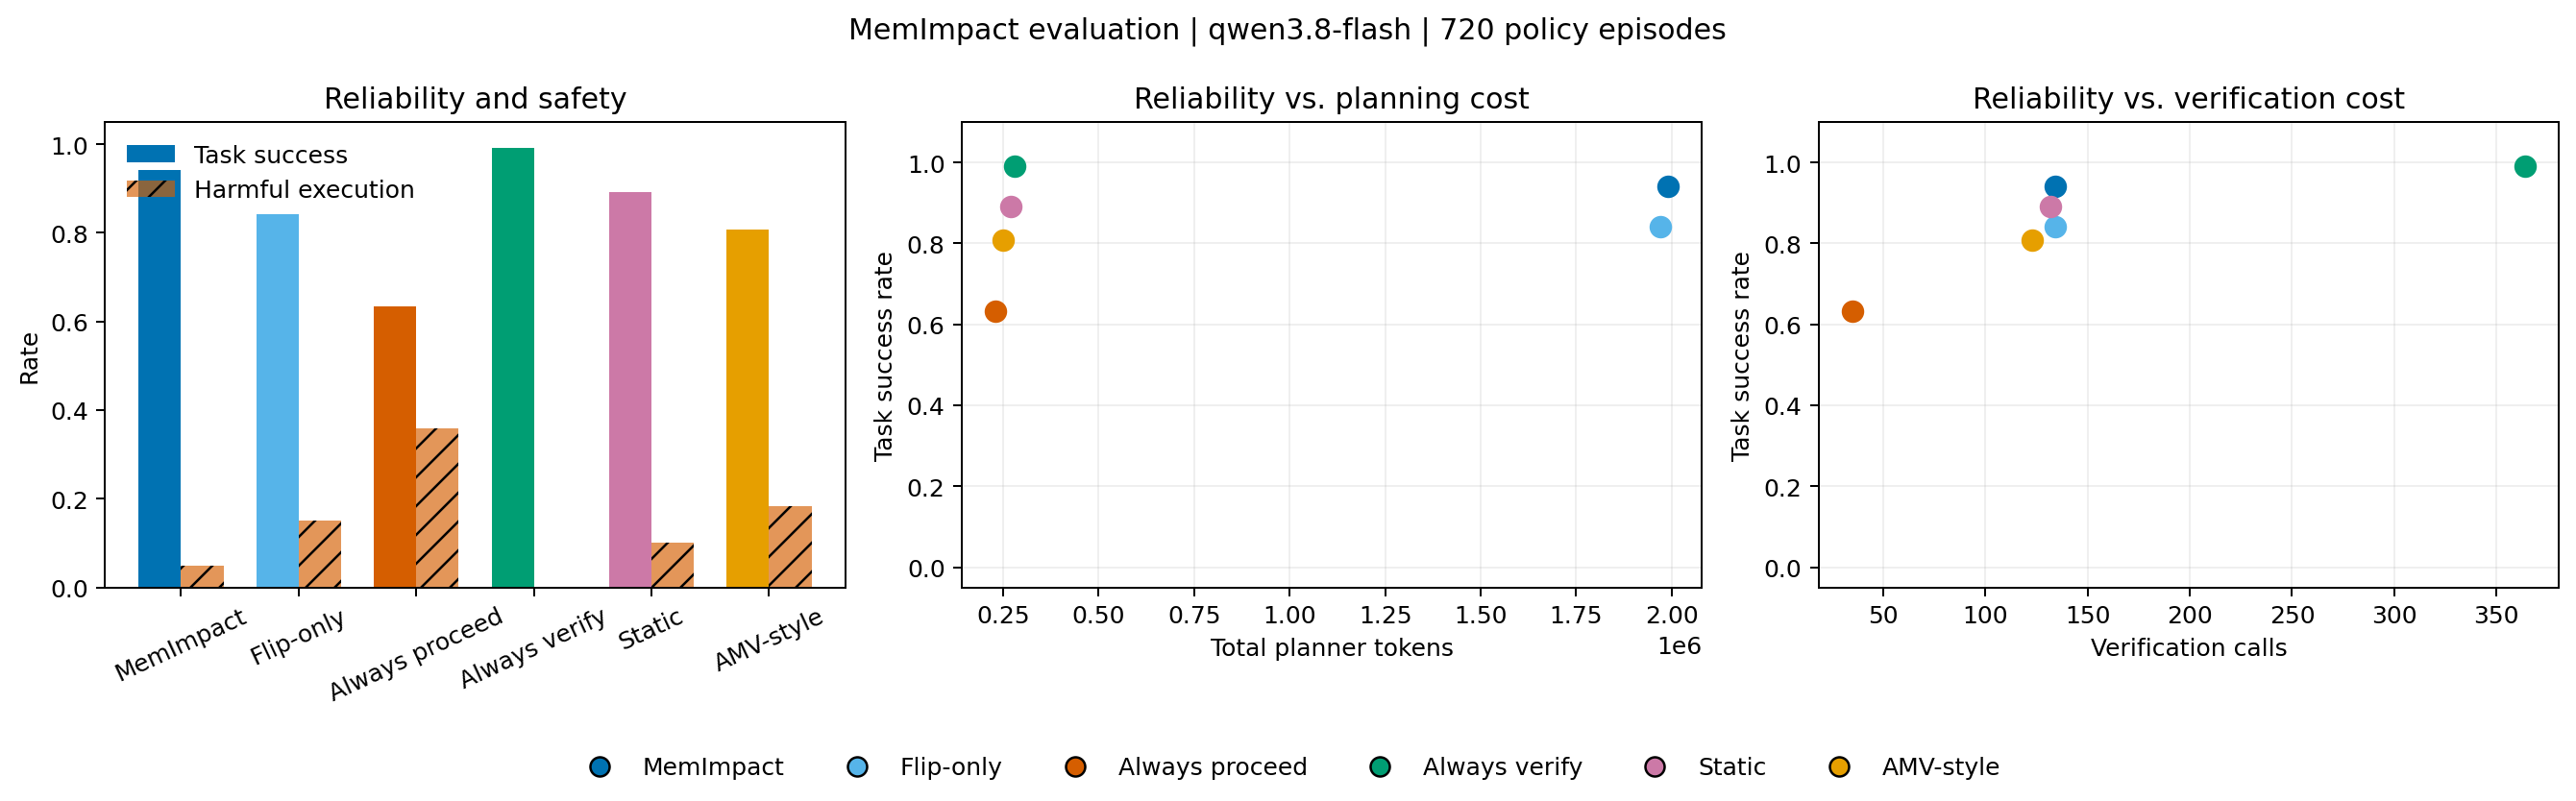
\includegraphics[width=0.98\textwidth]{../results/heldout/heldout_budget1_v1_langgraph_20261113_013824/reliability_cost.png}\\[0.5em]
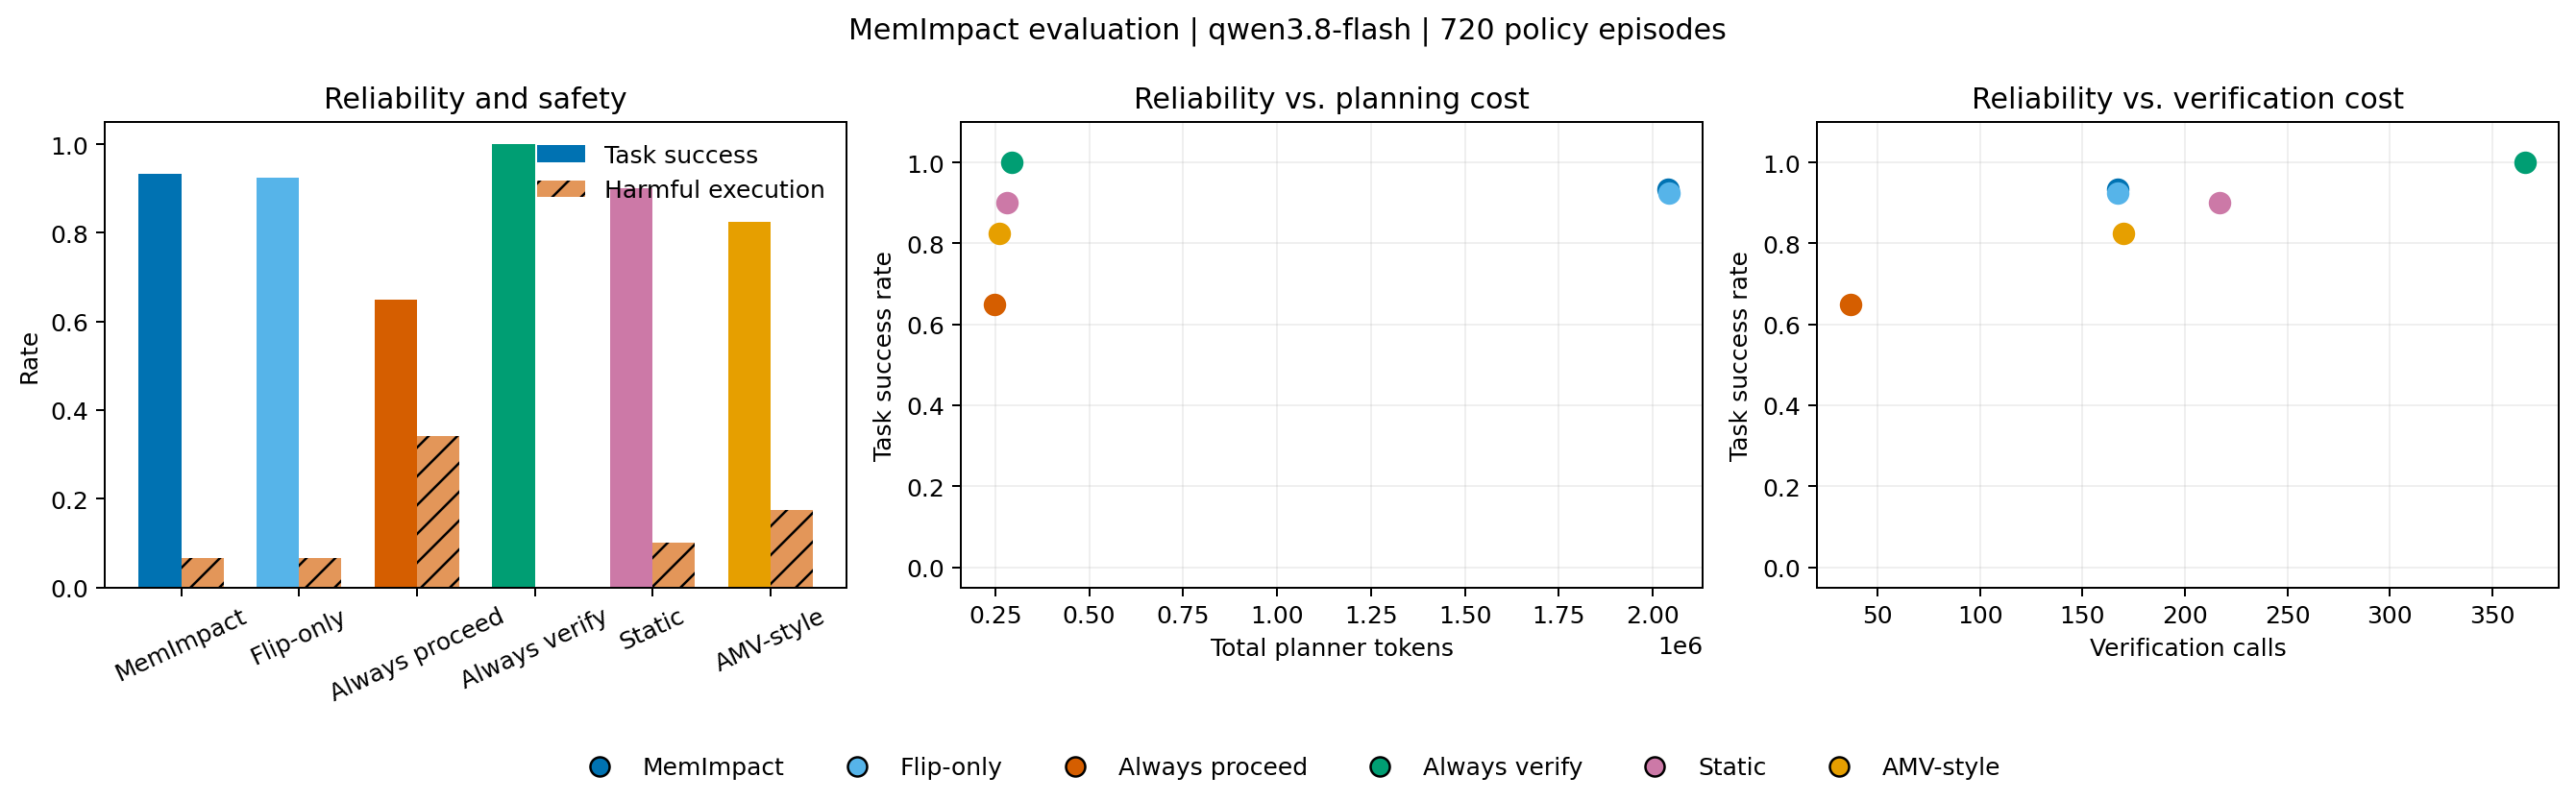
\includegraphics[width=0.98\textwidth]{../results/heldout/heldout_budget3_v1_langgraph_20261113_141753/reliability_cost.png}
\caption{Reliability and cost for \BOne (top) and \BThree (bottom). Each run contains 720 policy episodes.}
\label{fig:cost}
\end{figure}

Table~\ref{tab:paired} gives the paired success-rate differences. The \method advantage over flip-only is visible in \BOne but nearly disappears in \BThree. The AMV-style comparison follows the same attenuation, and its \BThree interval includes zero. Static remains competitive at much lower cost. Always Verify has higher reliability in both runs, with both observed bootstrap intervals excluding zero.

\begin{table}[t]
\centering
\small
\caption{Paired task-success differences: \method minus comparator. Values are percentage points with clustered 95\% bootstrap intervals.}
\label{tab:paired}
\begin{tabular}{lcc}
\toprule
Comparator & \BOne & \BThree \\
\midrule
Flip-only & +10.00 [3.33, 20.00] & +0.83 [0.00, 2.50] \\
Static & +5.00 [$-$3.33, 15.00] & +3.33 [$-$4.17, 12.50] \\
AMV-style & +13.33 [1.67, 25.00] & +10.83 [0.00, 21.67] \\
Always Verify & $-$5.00 [$-$10.00, $-$0.83] & $-$6.67 [$-$10.83, $-$2.50] \\
\bottomrule
\end{tabular}
\end{table}

\subsection{Direct and Indirect Dependence}

The strongest \BOne gains over flip-only occur in indirect deletion tasks, where full scoring selects a stale selection rule while flip-only verifies a concrete but wrong target mapping. Table~\ref{tab:dependence} shows that this pattern is not stable in \BThree: direct and indirect success are nearly identical for both counterfactual variants. Static and AMV-style remain perfect on direct tasks, where arguments expose the relevant memory, but lose reliability on indirect tasks.

\begin{table}[t]
\centering
\small
\caption{Task success (\%) by dependence type; each cell contains 60 episodes.}
\label{tab:dependence}
\begin{tabular}{lcccc}
\toprule
& \multicolumn{2}{c}{\BOne} & \multicolumn{2}{c}{\BThree} \\
\cmidrule(lr){2-3}\cmidrule(lr){4-5}
Policy & Direct & Indirect & Direct & Indirect \\
\midrule
\method & 95.00 & 93.33 & 93.33 & 93.33 \\
Flip-only & 95.00 & 73.33 & 93.33 & 91.67 \\
Always Verify & 98.33 & 98.33 & 100.00 & 100.00 \\
Static & 100.00 & 78.33 & 100.00 & 80.00 \\
AMV-style & 100.00 & 61.67 & 100.00 & 65.00 \\
\bottomrule
\end{tabular}
\end{table}

\subsection{Critical-Memory Identification}

Offline labeling finds 43 result-improving critical memories in \BOne and 41 in \BThree; each labeled scenario has at most one. The labels differ because the shared initial plans differ between independent runs. \method achieves high recall but low precision, and the full score and flip-only produce identical selections in \BThree (Table~\ref{tab:critical}). Thus, planner impact can find many useful checks but also triggers many checks whose verification does not improve the result.

\begin{table}[t]
\centering
\small
\caption{Critical-memory selection against outcome-improving offline labels.}
\label{tab:critical}
\begin{tabular}{lcccc}
\toprule
& \multicolumn{2}{c}{\BOne} & \multicolumn{2}{c}{\BThree} \\
\cmidrule(lr){2-3}\cmidrule(lr){4-5}
Policy & Precision & Recall & Precision & Recall \\
\midrule
\method & 0.363 & 0.860 & 0.232 & 0.805 \\
Flip-only & 0.245 & 0.581 & 0.232 & 0.805 \\
Static & 0.258 & 0.721 & 0.142 & 0.707 \\
AMV-style & 0.177 & 0.488 & 0.122 & 0.488 \\
Always Verify & 0.119 & 1.000 & 0.114 & 1.000 \\
\bottomrule
\end{tabular}
\end{table}

\subsection{Matched Budget Comparison}

Increasing selective-verification capacity does not monotonically improve outcomes (Table~\ref{tab:budget}). \method verifies 33 more memories or lookups in \BThree but has one fewer successful episode. Flip-only improves by ten successful episodes, yet its clustered interval includes zero. Static performs 85 additional checks for only one additional success. Since model calls are independent across runs, planner variability contributes to these changes; the table must not be read as an isolated budget treatment.

\begin{table}[t]
\centering
\small
\caption{Matched changes from \BOne to \BThree. Success differences are percentage points with clustered 95\% intervals; verification and token changes are run totals.}
\label{tab:budget}
\begin{tabular}{lrrr}
\toprule
Policy & $\Delta$ Success [CI] & $\Delta$ Verify & $\Delta$ Tokens \\
\midrule
\method & $-$0.83 [$-$4.17, 2.50] & +33 & +47,984 \\
Flip-only & +8.33 [$-$1.67, 20.00] & +33 & +72,750 \\
Always Proceed & +1.67 [$-$1.67, 5.00] & +2 & +19,160 \\
Always Verify & +0.83 [0.00, 2.50] & +2 & +14,367 \\
Static & +0.83 [0.00, 2.50] & +85 & +11,597 \\
AMV-style & +1.67 [$-$1.67, 5.00] & +47 & +12,498 \\
\bottomrule
\end{tabular}
\end{table}

Abstention is almost absent: all \BOne policies abstain on zero episodes, while \BThree has one flip-only and one Always Proceed abstention. Proceed coverage and safe-proceed recall therefore provide little discrimination in this implementation. We do not use them as evidence of superiority.

\section{Case Studies}

\subsection{Success: Verifying an Indirect Selection Rule}

In \texttt{heldout\_deletion\_lecture\_stale\_low} under \BOne, the user asks to delete the guest-lecture reminder using a stored mapping. A stale rule instead says to delete the library-book reminder, and the initial action follows that rule. Removing either \texttt{mem\_rule} or \texttt{mem\_other} flips all three paired actions, so flip-only ties them and selects \texttt{mem\_other}. That check confirms the library-book mapping, after which the wrong reminder is deleted.

Full \method gives \texttt{mem\_rule} a slightly higher score (1.988 versus 1.974) because it is older. Verification refutes the rule, replanning selects the guest-lecture ID, and execution succeeds without harmful deletion. This case demonstrates how non-impact terms can resolve a flip tie. It is not evidence of general superiority: Static also solves the case, and \method uses 24,321 planner tokens.

\subsection{Failure: Verifying a True Premise of a Wrong Action}

In \texttt{heldout\_messaging\_riley\_misattributed\_low} under \BThree, the agent should use Riley's personal number, but a misattributed rule says to use the work channel. Full-memory planning is unstable ($\widehat F_0=0.667$). Removing the rule has raw flip rate 0.667, so its noise-adjusted impact is zero. Removing the work-number memory has adjusted impact 0.333, so the policy verifies that number.

The work number is confirmed as a real record, but the routing rule remains wrong, and the agent sends to the work number. Always Verify checks all three memories, refutes the routing rule, and sends correctly. It uses 2,810 tokens versus 16,239 for \method in this episode. The failure shows both the limitation of subtracting a high variability baseline and the difference between verifying an action argument and verifying the rule that selected it.

\subsection{Unnecessary Verification: Action Flips Without Outcome Benefit}

In \texttt{heldout\_messaging\_morgan\_irrelevant\_low} under \BThree, the initial action already uses the correct number and message. Removing the phone, brief-message preference, or coffee preference changes the proposed action often enough to give all three positive impact scores. \method exhausts its budget and verifies all three; the offline label set is empty because none of these checks is needed to improve the result.

The final message is correct, but the episode uses three verification calls and 14,782 planner tokens. Always Proceed completes the same task with zero verification and 1,315 tokens. This case illustrates why action influence is not equivalent to verification value, and why a larger budget can increase unnecessary checks without improving the outcome.

\section{Discussion}

\paragraph{RQ1: Critical-memory identification.} Planner-level auditing obtains high recall, but low precision and substantial run variability prevent a claim of consistently superior identification. In \BOne it outrecalls flip-only, Static, and AMV-style; in \BThree its selection metrics are identical to flip-only. Always Verify obtains perfect recall with lower precision by checking every memory. More importantly, high recall for \method comes with many non-critical checks.

\paragraph{RQ2: Reliability--cost trade-off.} The results do not support the hypothesis that planner re-execution improves the overall trade-off. It reduces harm relative to acting without verification and checks fewer memories than Always Verify, but Always Verify is more reliable and substantially cheaper in planner tokens and latency. Static is also competitive at much lower cost. Any advantage is therefore local to particular indirect cases, not an overall Pareto improvement.

\paragraph{RQ3: Dependence and budget conditions.} Indirect dependence exposes a genuine weakness of literal candidate-conditioned auditing, and \BOne shows a meaningful advantage over flip-only there. However, \BThree does not reproduce the same magnitude. Increasing the verification cap from one to three improves flip-only descriptively but not \method, and all cross-budget success intervals for the selective methods include zero. More budget can simply mean more unnecessary verification.

\section{Limitations}

The benchmark is synthetic and contains only two held-out task families and twelve base-scenario clusters. Results from one hosted model do not establish transfer to other planners. Three fixed memories, authoritative verification overrides, and at most one state-changing action simplify real memory and tool-use settings. The verifier supplies correct evidence by construction; noisy or incomplete verification remains untested.

The AMV-style baseline uses literal argument overlap rather than AMV-Guard's full method, and Static uses task-relevant scopes and age. Conclusions about these baselines apply only to these adaptations. The full score's age/provenance weighting is only one instantiation, so the flip-only comparison does not evaluate all possible scoring functions. Leave-one-out removal can miss redundant or interacting memories, and noise subtraction can hide a critical memory when baseline variability is high.

The two budgets were run independently rather than with shared traces across budgets, preventing a strict causal estimate of budget effects. Bootstrap intervals describe variability within this clustered benchmark, not broad population uncertainty. Token usage excludes monetary pricing, and latency excludes verification-tool execution. Finally, harm covers only outcomes encoded by the simulator; the method is not a general safety guarantee.

\section{Conclusion}

We implemented a reproducible planner-level counterfactual memory-auditing pipeline and compared it with five alternatives on two frozen 120-episode evaluations. The method can identify and correct indirect memory-driven errors, but its benefits are inconsistent across independent runs and its planning overhead is substantial. Always Verify provides the strongest reliability at far lower planner cost, while Static remains a strong low-cost comparator. The main answer to our research question is therefore negative for the overall benchmark: planner re-execution has localized value, but we do not observe a reliable overall reliability--cost improvement. Future work should test learned verification value, redundant-memory interventions, noisier evidence, and shared-trace budget controls before recommending planner-level auditing for deployment.

\section*{Reproducibility}

The \href{https://github.com/junjiacaohku-ai/COMP7607-Group-Project-MemImpact}{public GitHub repository} contains all artifacts. The following commands reproduce model runs, offline labels, single-run analyses, and the matched comparison. Model runs require locally configured credentials; credentials are not stored in the repository.

\begin{verbatim}
.venv/bin/python scripts/run_langgraph_comparison.py \
  --config configs/heldout_budget1_v1.yaml
.venv/bin/python scripts/run_langgraph_comparison.py \
  --config configs/heldout_budget3_v1.yaml
.venv/bin/python scripts/generate_critical_labels.py RUN_DIRECTORY
.venv-toolsandbox/bin/python scripts/analyze_comparison.py \
  RUN_DIRECTORY/comparison_summary.json
.venv/bin/python scripts/compare_verification_budgets.py \
  results/heldout/heldout_budget1_v1_langgraph_20261113_013824 \
  results/heldout/heldout_budget3_v1_langgraph_20261113_141753
\end{verbatim}

\appendix
\section{Additional Grouped Results}

Tables~\ref{tab:condition} and \ref{tab:consequence} report task success by memory condition and consequence. Each condition cell contains 24 episodes; each consequence cell contains 60. Conflicting and valid memories are largely solved by all methods, while stale and misattributed memories expose the largest differences. The single \BOne irrelevant-case failure shared across policies is the invalid reminder-ID execution error.

\begin{table}[h]
\centering
\scriptsize
\caption{Task success (\%) by memory condition for \BOne / \BThree.}
\label{tab:condition}
\begin{tabular}{lrrrrrr}
\toprule
Condition & \method & Flip & Proceed & Verify & Static & AMV \\
\midrule
Valid & 100 / 100 & 100 / 100 & 100 / 100 & 100 / 100 & 100 / 100 & 100 / 100 \\
Stale & 83.3 / 83.3 & 58.3 / 83.3 & 8.3 / 8.3 & 100 / 100 & 75.0 / 75.0 & 58.3 / 50.0 \\
Conflicting & 100 / 100 & 100 / 95.8 & 100 / 100 & 100 / 100 & 100 / 100 & 100 / 100 \\
Misattributed & 91.7 / 83.3 & 66.7 / 83.3 & 12.5 / 16.7 & 100 / 100 & 75.0 / 75.0 & 50.0 / 62.5 \\
Irrelevant & 95.8 / 100 & 95.8 / 100 & 95.8 / 100 & 95.8 / 100 & 95.8 / 100 & 95.8 / 100 \\
\bottomrule
\end{tabular}
\end{table}

\begin{table}[h]
\centering
\scriptsize
\caption{Task success (\%) by consequence level for \BOne / \BThree.}
\label{tab:consequence}
\begin{tabular}{lrrrrrr}
\toprule
Level & \method & Flip & Proceed & Verify & Static & AMV \\
\midrule
Low & 93.3 / 91.7 & 83.3 / 91.7 & 65.0 / 66.7 & 100 / 100 & 90.0 / 90.0 & 83.3 / 81.7 \\
High & 95.0 / 95.0 & 85.0 / 93.3 & 61.7 / 63.3 & 98.3 / 100 & 88.3 / 90.0 & 78.3 / 83.3 \\
\bottomrule
\end{tabular}
\end{table}

\section{Claim-to-Artifact Appendix}

\begingroup\footnotesize
All paths below are relative to the repository root. In Table~\ref{tab:artifacts}, \path{B1/} denotes \path{results/heldout/heldout_budget1_v1_langgraph_20261113_013824/}, and \path{B3/} denotes \path{results/heldout/heldout_budget3_v1_langgraph_20261113_141753/}. Raw per-scenario traces provide the underlying planner calls and attempts.\par
\endgroup

\begin{table}[h]
\centering
\scriptsize
\caption{Claim-to-artifact map.}
\label{tab:artifacts}
\begin{tabularx}{\textwidth}{p{0.25\textwidth}X}
\toprule
Claim or output & Evidence \\
\midrule
Overall metrics, both budgets & \path{B1/comparison_summary.json} and \path{B3/comparison_summary.json} \\
Grouped success and cost & \path{grouped_metrics.csv} and \path{per_episode_metrics.csv} in each run directory \\
Paired policy intervals & \path{paired_bootstrap.json} in each run directory \\
Critical-memory metrics & \path{critical_memory_metrics.json} and per-scenario \path{critical_labels.json} \\
Matched budget changes & \path{B3/budget_matched_comparison.json} \\
Successful indirect case & \path{B1/heldout_deletion_lecture_stale_low/memimpact/result_summary.json} \\
Wrong-premise failure & \path{B3/heldout_messaging_riley_misattributed_low/memimpact/result_summary.json} \\
Unnecessary verification & \path{B3/heldout_messaging_morgan_irrelevant_low/memimpact/result_summary.json} \\
Configuration and integrity & \path{run_metadata.json}, \path{resume_history.json}, and \path{configs/heldout_budget1_v1.yaml} / \path{heldout_budget3_v1.yaml} \\
Implementation & \path{memimpact/langgraph_runtime.py}, \path{memimpact/core.py}, \path{memimpact/scoring.py}, and \path{scripts/run_langgraph_comparison.py} \\
\bottomrule
\end{tabularx}
\end{table}

The configuration and environment hashes are:
\begingroup\footnotesize
\begin{verbatim}
Budget-1 config: 54665697d88417deb40b27534ea4b6da2e0347f2f0253733c0f8a3afc037a50f
Budget-3 config: c4719d8c1296e9e3fb7968c3214de281964543f2d761d52bb171bc10b16dd778
ToolSandbox:     c8571d7854316d2e1c5f288e59fe1e34e53f6dd1
\end{verbatim}
\endgroup
Both runs record the same planner-prompt and tool-schema hashes. Offline labeling uses 146 attempts and 195,516 tokens for \BOne, and 154 attempts and 206,606 tokens for \BThree; these costs are separate from Table~\ref{tab:main}.

\bibliographystyle{plainnat}
\bibliography{../proposal/references}

\end{document}
